%\documentclass[review]{cvpr}
\documentclass[final]{cvpr}

\usepackage{times}
\usepackage{epsfig}
\usepackage{graphicx}
\usepackage{amsmath}
\usepackage{amssymb}
% \documentclass{article}
\usepackage{array}
\usepackage{graphicx}
\usepackage{multirow}
\newcommand\MyBox[2]{
  \fbox{\lower0.75cm
    \vbox to 1.7cm{\vfil
      \hbox to 1.7cm{\hfil\parbox{1.4cm}{#1\\#2}\hfil}
      \vfil}%
  }%
}
%Path relative to the main .tex file 
\graphicspath{ {./images/} }
% Include other packages here, before hyperref.

% If you comment hyperref and then uncomment it, you should delete
% egpaper.aux before re-running latex.  (Or just hit 'q' on the first latex
% run, let it finish, and you should be clear).
\usepackage[pagebackref=true,breaklinks=true,colorlinks,bookmarks=false]{hyperref}


\def\cvprPaperID{****} % *** Enter the CVPR Paper ID here
\def\confYear{CVPR 2021}
%\setcounter{page}{4321} % For final version only


\begin{document}

%%%%%%%%% TITLE
\title{Survey On Machine Learning Paradigms For Phishing Website Detection}

\author{Madan Baduwal\textsuperscript{1}  \and Prakash Madai\textsuperscript{2} \and Tasnimul Alam \textsuperscript{3} \and Quan Yuan \textsuperscript{4} \\
\textsuperscript{\rmfamily\textbf{}}Department of Computer Science, University of Texas Permian Basin\\
\texttt{\{baduwal\textunderscore m63609,madai\textunderscore p57558,alam\textunderscore m61291,yuan\textunderscore q\}@utpb.edu}}


\maketitle


%%%%%%%%% ABSTRACT
\begin{abstract}
   Phishing attacks continue to be a major security threat for individuals and organizations alike. It causes billions of dollars in losses annually. Machine learning(ML) has shown great promise in detecting such attacks by identifying patterns and anomalies in large datasets. The tradeoff between feature selection and model selection is a tedious task in ML for phishing detection. Low number of features are not enough for the generalizability of traditional machine learning algorithms i.e.For Logistic Regression(LR), Support Vector Machine(SVM), Random Forest(RF), XG boost and Naive Bayes(NB). And it's tough for deep learning(DL) algorithms to learn features from ambiguities behaviour between phishing and non-phishing websites. This paper presents a comprehensive survey of various ML and ML paradigms that have been employed for the detection of phishing websites. The survey also discusses various datasets, features, number of parameters in algorithms, training time-space complexity in phishing detection and compares the accuracies of different ML techniques. The results of this survey provide valuable insight into the current state of the art in phishing detection and can serve as a useful resource for researchers and practitioners working in this field.

\end{abstract}

\textbf{Keywords:} Phishing Detection, Machine Learning, Deep Learning, Cyber Security, Cybercrime

%%%%%%%%% BODY TEXT
\section{Introduction}

As of January 2023, there were 5.16 billion individuals worldwide were using the internet, accounting for 64.4\% of the global population. Of this figure, 4.76 billion people, or 59.4\% of the world's population, were utilizing social media platforms~\cite{Authors01}. The internet has revolutionized various aspects of people's lives, including communication, shopping, chatting, and office work. With the onset of the pandemic in late 2019, many conventional industries have transitioned from offline to online services, such as retail, catering, Education, Entertainment, Healthcare, and Banking and Finance.


Phishing websites have become a significant threat to online security. These fraudulent websites are created with the intent of deceiving users into disclosing their confidential information, such as passwords, credit card details, and other sensitive personal data~\cite{Authors02}. Phishing attacks are executed using several tactics such as link manipulation, filter evasion, website forgery, covert redirect, and social engineering. Spoofing web pages that mimic legitimate websites are the most common approach used in these attacks. They are considered a significant threat and were among the top concerns highlighted in the 2022 Internet Crime Report issued by the U.S. Federal Bureau of Investigation's Internet Crime Complaint Center (IC3). The IC3's statistics for 2022 revealed that internet-based theft, fraud, and exploitation remain widespread, resulting in a massive \$10.3 billion in financial losses that year. The IC3 received a staggering 800,944 complaints related to business email compromise (BEC) and email account compromise (EAC) in 2022. ~\cite{FBI-IC3}
.  

\hspace*{-0.2in}
\begin{figure}[h]
   \centering
   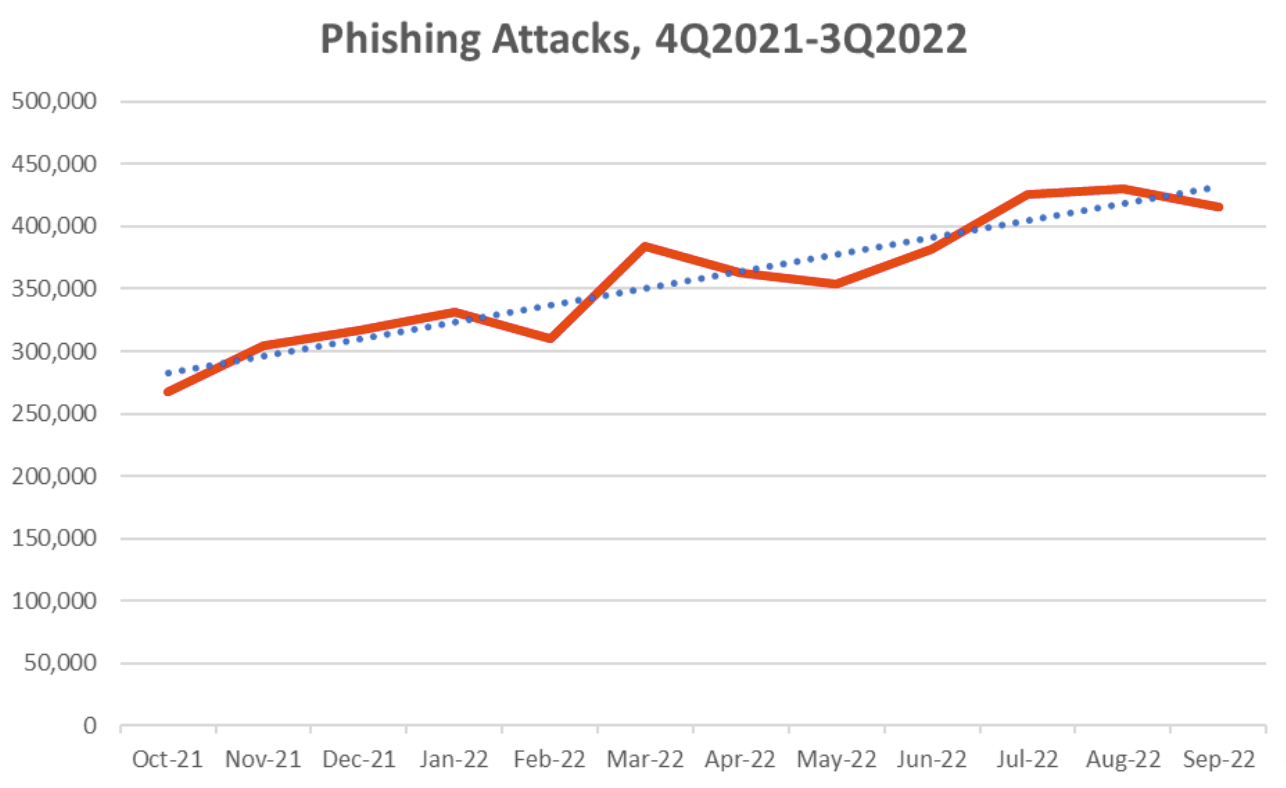
\includegraphics[width=8cm, height=5cm]{APWG-phishing-detection-report.png}
   \caption{Total number of phishing websites detected by APWG}
   \label{fig:apwg-report}
\end{figure}

Anti-Phishing Working Group(APWG) emphasizes that phishing attacks have grown in recent years, Figures~\ref{fig:apwg-report} illustrates the total number of phishing sites detected by APWG in the first quarter of 2022 and the last quarter of 2021. During the third quarter of 2022, APWG recorded a staggering 1,270,883 phishing attacks, marking a new record and the most severe quarter for phishing observed by APWG to date. The total for August 2022 was 430,141 attacks, which is the highest monthly total reported. The number of reported phishing attacks reported to APWG has more than quintupled since the first quarter of 2020, when APWG observed 230,554 attacks. The rise in Q3 2022 is attributable in part to increasing numbers of attacks reported against several specific targets. These targets suffered from large numbers of attacks from persistent phishers. Statistical Highlights for the 3rd Quarter 2022~\cite{APWG-Report}.

With the increasing sophistication of phishing attacks, conventional anti-phishing techniques are becoming less effective. To address this problem, machine learning has emerged as a promising solution for real-time detection of phishing websites. Our study has examined several machine learning methods, including Logistic Regression, KNN, Support Vector Machine, Random Forest, Ada-Boost, Gradient Boosting, XGBoost, Naive Bayes, Feed Forward Neural Networks, Convolution Neural Networks (CNN), Recurrent Neural Networks (RNN), and Transformers~\cite{Machine-learning-algorithms}. 

The following sections of the paper are arranged in the following manner. In section \ref{sec:Phishing Techniques} we list some
widely used phishing techniques,  in Section \ref{sec:Phishing Detection Approaches} we discuss different types of phishing and phishing attack prevention methods, Section \ref{sec:Background and Related Work} reviews the background and related work of phishing, in section \ref{sec:Datasets} we discuss the datasets usually used in machine learning approaches, Section \ref{sec:Preprocessing And Feature Engineering} reviews the preprocessing and feature engineering that usually use in machine learning for phishing detection. Section \ref{sec:Machine Learning Approach} lists the methodologies of detecting website phishing in regards to approaches, this includes techniques based on machine learning methods. Specifically, we provide a detailed explanation of the overall architecture of the machine learning-based solution for detecting phishing networks. In section \ref{sec:Evaluation Matrices}
 we show evaluation results of suggested machine learning subsequently, we conclude by discussing future implications and insights stemming from the methods used \ref{sec:Conclusion}.



Furthermore, the paper will provide a critical analysis of the current state-of-the-art, identifying the strengths and weaknesses of each machine learning paradigm in phishing detection. Finally, the survey will conclude by discussing the challenges and future research directions in machine learning-based anti-phishing techniques.

In conclusion, this paper's primary objective is to provide a comprehensive survey of machine learning paradigms for phishing website detection. The survey will be useful for researchers, practitioners, and policymakers in the field of cybersecurity, providing insights into the latest trends and developments in machine learning-based antiphishing techniques.

\section{Phishing Techniques}
\label{sec:Phishing Techniques}
This section covers various phishing techniques that are commonly employed by criminals to trick individuals.

\subsection{Link manipulation}

Phishing primarily revolves around links, with attackers utilizing various  techniques to deceive users into clicking on them. One such technique involves manipulating the URL to mimic a legitimate one, such as representing malicious URLs as hyperlinks with legitimate names on websites. Another approach is to create misspelled URLs that closely resemble legitimate ones, for instance, facebuuk.com. However, there is a much more sophisticated variant of typosquatting known as IDN Spoofing, which involves the use of non-English characters that bear a striking resemblance to their English counterparts. For example, an attacker might use a Cyrillic "c" or "a" instead of the corresponding English letters, making it significantly more difficult to recognize the deception~\cite{VB2018}.

\subsection{Filter evasion}

Phishers often display the content of their fraudulent websites as images or use Adobe Flash to make it challenging for some phishing detection techniques to detect their malicious activities. To counter this type of attack, optical character recognition (OCR) technology must be employed ~\cite{lam2009counteracting}.

\subsection{Website forgery}

In this form of attack, phishers manipulate the JavaScript code of a legitimate website to carry out phishing activities. These types of attacks, also referred to as cross-site scripting, are exceptionally difficult to detect since the victim is interacting with a genuine website~\cite{lam2009counteracting}.

\subsection{Covert redirect}

This attack is aimed at websites that use the OAuth 2.0 and OpenID protocols. In this scenario, when attempting to grant token access to a legitimate website, users inadvertently provide their token to a malicious service.  Nevertheless, this technique has received little attention due to its limited significance ~\cite{Waziri20151WF}.

\subsection{Social engineering}

Social engineering phishing is a deceptive attack that employs psychological manipulation to trick users into divulging their security information. This type of attack typically involves multiple steps: first, the phisher researches the potential vulnerabilities of their targets. Next, the phisher attempts to gain the target's trust before finally creating a situation where the target unwittingly discloses important information. Social engineering phishing techniques include baiting, scareware, pretexting, and spear phishing ~\cite{krombholz2015advanced}.

\section{Phishing Detection Approaches}
\label{sec:Phishing Detection Approaches}

There have been several proposed methods to prevent phishing attacks across each stage of the attack flow. Some of these methods involve training users to recognize and prepare for future attacks, while others operate automatically to alert and protect the user~\cite{phishing-detection}. The following methods can be categorized as follows:

\subsection{Rule-based Approaches}
Rule-based approaches use a set of predefined rules or heuristics to identify and block phishing websites. These rules are typically based on known patterns and characteristics of phishing attacks, such as URL or domain name similarity to legitimate websites, suspicious keywords, and IP reputation ~\cite{phishing-detection1}.

One of the advantages of rule-based approaches is that they are relatively simple and can be easily implemented. However, they are not very effective against new and sophisticated phishing attacks that may not fit into the predefined rules.

\subsection{Signature-based Approaches}
Signature-based approaches use signatures or fingerprints of known phishing attacks to identify and block new phishing websites. These signatures can be based on various factors such as URLs, IP addresses, email addresses, and content.

The advantage of signature-based approaches is that they are very effective at detecting known phishing attacks. However, they may not be effective against new and previously unseen phishing attacks.

\subsection{Machine Learning Approaches}
Machine learning algorithms can be used to detect phishing attacks by analyzing various features such as website content, URL structure, IP address, and user behavior. Machine learning algorithms can detect previously unseen phishing attacks by learning from a large dataset of known phishing attacks~\cite{shahrivari2020phishing}.

Some of the commonly used machine learning algorithms for phishing detection include Logistic Regression, Support Vector Machine (SVM), Random Forest, Gradient Boosting, Naive Bayes, Feed Forward Neural Networks, Convolution Neural Networks (CNN), Recurrent Neural Networks (RNN), and Transformers.

The advantage of machine learning approaches is that they can adapt to new and previously unseen phishing attacks, making them more effective than rule-based and signature-based approaches. However, machine learning algorithms require a large amount of data for training and may produce false positives and false negatives.

\subsection{Hybrid Approaches}
Hybrid approaches combine multiple detection techniques to improve accuracy and reduce false positives. For example, a hybrid approach might use rule-based techniques to quickly identify known phishing websites and machine learning algorithms to detect previously unseen attacks.

The advantage of hybrid approaches is that they can provide better protection against phishing attacks than a single detection technique. However, they can be more complex to implement and require more computational resources ~\cite{phishing-detection2}.

\subsection{User Education}
Educating users about the risks and warning signs of phishing attacks can help them to identify and avoid phishing websites. This approach relies on user awareness and vigilance rather than technology-based detection methods.

The advantage of user education is that it can be effective in preventing phishing attacks if users are well-informed and cautious. However, it may not be effective against new and sophisticated phishing attacks that exploit human vulnerabilities.

\section{Background and Related Work}
\label{sec:Background and Related Work}

Figure~\ref{fig:phishinglifecycle}  depicts the life cycle of a typical phishing attack. Phishing attacks often start with an attacker sending a fraudulent email or message that appears to be from a trusted source, such as a bank or a social media website. The email or message contains a link that directs the victim to a phishing website, which is designed to look like a legitimate website. The victim is then prompted to enter their sensitive information, such as login credentials, credit card information, or personal details. Once the victim submits their information, it is collected by the attacker for financial gain or other malicious purposes.


\hspace*{-0.2in}
\begin{figure}[h]
   \centering
   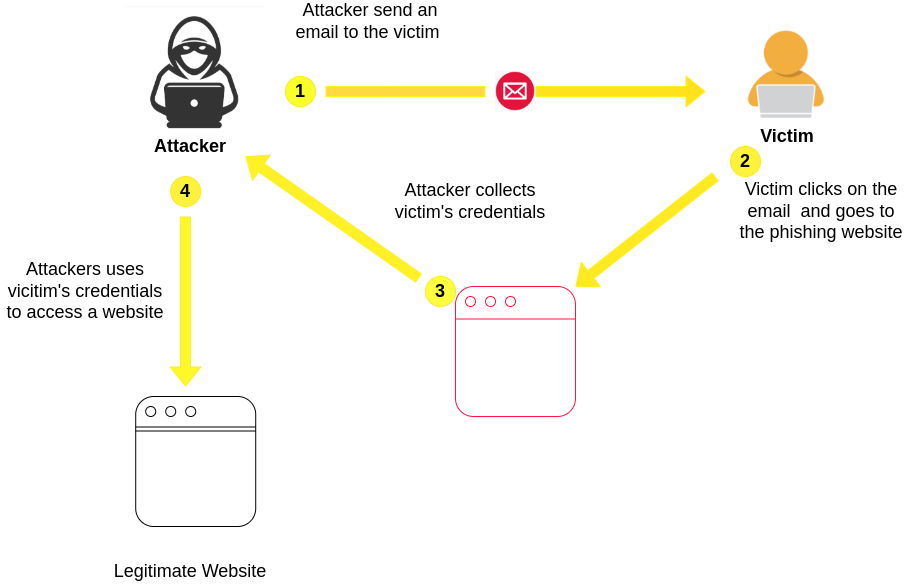
\includegraphics[width=8cm, height=5cm]{phishing-life-cycle.png}
   \caption{Phishing Life Cycle}
   \label{fig:phishinglifecycle}
\end{figure}

First, an attacker creates a phishing website that looks very similar to a legitimate website. Attackers use various methods to forge the URL of a legitimate website, particularly the domain name and network resource directory, including using spelling mistakes, similar alphabetic characters, and other techniques. For example, the link “https://aimazon.amz-z7acyuup9z0y16.xyz/v”,imitates https://www.amazon.com. More details about phishing techniques are in section \ref{sec:Phishing Techniques}. This means that while the URL of a phishing website may be visible to the user by hovering over the link, it can still be challenging for an average user to recognize it as a fake URL that imitates a legitimate one. Additionally, cybercriminals often use scripts to obtain logos, web layouts, and text from genuine web pages, which allows them to create phishing websites that closely resemble legitimate ones. As a result, imitation of web content is also a crucial factor in successful phishing attacks. Attackers often use scripts to copy the logos, web layouts, and text from genuine web pages to make the phishing website look as similar as possible to the legitimate website. They also often create fake form submission pages that ask users to input sensitive information such as login credentials, payment information, and password recovery information. These pages are designed to look exactly like the legitimate pages, in order to trick users into giving away their sensitive information.

In the second step, attackers rely heavily on social engineering tactics to manipulate users into clicking on the phishing link. They often use fear and urgency to create a sense of pressure on the user, such as threatening to suspend their account or urging them to take immediate action to avoid a negative consequence. They may also try to gain the user's trust by impersonating a familiar brand or authority figure. Phishing attacks can be delivered through various channels, including email, SMS, voice messages, QR codes, and spoof mobile applications. In some cases, attackers may use multiple channels to increase their chances of success. Once the user clicks on the phishing link, they will be directed to a fake website that looks similar to the legitimate one. Attackers often use scripts to obtain logos, web layouts, and text from genuine web pages to make the fake website look more convincing. The user may be prompted to enter sensitive information, such as their login credentials or payment details, which will be collected by the attacker.


The next step is users submit their personal information, such as login credentials, payment information, and other sensitive data on the fake website, attackers will receive all the information. This is a critical step in the phishing process as it allows the attackers to gain access to the user's accounts or use the information for fraudulent purposes. It's important for users to be cautious and verify the authenticity of websites before submitting any sensitive information.

The final stage involves the utilization of a user's genuine details to fabricate a genuine website request, resulting in the misappropriation of the user's account funds. It is common for people to use identical login credentials across various websites, enabling the attacker to pilfer multiple accounts from a single individual. Some cybercriminals employ stolen data for unlawful pursuits. Phishing tactics have evolved since their inception in 1987, keeping pace with the advancements in internet technology. As online payment mechanisms gained popularity, attackers shifted their focus to online payment phishing. The article "A comprehensive survey of AI-enabled phishing attacks detection techniques," published in 2020 in the Telecommunications Systems journal, discusses different methods that use artificial intelligence (AI) to detect phishing attacks. These attacks involve the impersonation of a trustworthy entity to steal sensitive information from individuals or organizations. The authors conducted a survey of recent research papers and categorized the techniques into rule-based, machine learning-based, hybrid, and deep learning-based~\cite{basit2020comprehensive}. They emphasized the importance of using AI-based techniques to improve phishing attack detection, as traditional approaches may not be effective against increasingly sophisticated attempts. The article also suggests future research directions, such as developing techniques to detect zero-day phishing attacks and considering user behavior and contextual information. Overall, the article provides a useful resource for those interested in developing and implementing AI-enabled phishing attack detection techniques. In "Phishing Detection: A Machine Learning Approach," Singh et al. reviewed machine learning-based techniques for detecting phishing attacks~\cite{singh2020phishing}. The authors provided an overview of the history of phishing and highlighted major phishing attack reports. They classified phishing attacks into two types: social engineering attacks and malware-based phishing. The authors also categorized features into three groups: source code features, URL features, and image features. These feature categories were rule-based and used to detect phishing attacks.

In 2020, Vijayalakshmi et al. conducted a survey on major detection techniques and a taxonomy for detecting phishing in their research paper~\cite{vijayalakshmi2020web}. They referred to a statistical report from APWG to illustrate the trend of phishing attacks between 2017 and 2019. The paper introduced a taxonomy of automated phishing detection solutions, which classified the solutions into three categories based on the input parameters: web address-based methods, webpage content-based solutions, and hybrid approaches. The web address-based approaches were further divided into list-based, heuristic rule-based, and learning-based approaches, while web content-based solutions were categorized into rule-based and machine learning-based solutions. The authors listed most of the state-of-the-art methodologies for each category and presented the details of each solution. They then compared all the methods based on several evaluation metrics, such as classification performance, limitations, third-party service independence, and zero-hour attack detection. Finally, the authors suggested that hybrid approaches would achieve high accuracy rates and be suitable for real-time systems, and deep learning-based solutions would be a promising direction for future research.


Kalaharsha and Mehtre conducted a survey on phishing detection solutions, which were classified into multiple categories based on the techniques and input parameters used, in their research paper titled "Detecting Phishing Attacks: A Survey." The authors introduced different types of phishing attacks and three phishing techniques~\cite{kalaharsha2021detecting}. They listed 18 methods and 9 datasets for detecting phishing websites and compared the accuracy performance of all the models. Furthermore, the paper presented some challenges, such as reducing false-positive rates and overfitting, in detecting phishing attacks.


The paper by Jain and Gupta, titled "A Comprehensive Survey on Analyzing Phishing Attack Techniques, Detection Methods, and Some Existing Challenges" provides a detailed overview of phishing attack techniques, detection methods, and challenges associated with combating phishing attacks~\cite{jain2021survey}. The authors gather statistical reports on the prevalence and motivation behind phishing attacks and describe various techniques that attackers use to target both PCs and smartphones.In the paper, the authors also present different defense methods that have been proposed to detect and prevent phishing attacks. They analyze and compare existing anti-phishing approaches published from 2006 to 2017, highlighting their advantages and limitations.
Towards the end of the paper, Jain and Gupta discuss several major challenges associated with detecting and preventing phishing attacks, such as selecting efficient features, identifying tiny URLs, and detecting attacks on smartphones. Overall, the paper provides a comprehensive overview of the state-of-the-art techniques for detecting and preventing phishing attacks, and highlights the need for further research in this area to address the remaining challenges.

A recent paper "Phishing or Not Phishing? A Survey on the Detection of Phishing Websites" by Rasha Zieni, Luisa Massari, and Maria Carla Calzarossa investigates the effectiveness of different methods for detecting phishing websites ~\cite{zieni2019phishing}. The authors conducted a survey to evaluate the accuracy of several approaches, including machine-learning techniques, feature-based techniques, and heuristic methods. They found that the combination of several techniques is necessary to achieve a high level of accuracy in detecting phishing websites. They also identified some challenges in this field, such as the need for a large and diverse dataset of phishing websites and the difficulty of staying up-to-date with the constantly evolving phishing techniques. The paper provides insights that could help researchers and practitioners develop better methods for detecting phishing websites.

\section{Datasets}
\label{sec:Datasets}

Each approach relies on data as its source and this data is a critical factor in determining its performance. In other words, the quality and quantity of the data used to develop and test an approach heavily influence its accuracy and effectiveness. Therefore, obtaining reliable and relevant data is essential to achieving positive outcomes in any data-driven approach. There exist two approaches for data collection: utilizing published datasets and extracting data by retrieving URLs directly from the internet. Table ~\ref{tab:dataset} shows several major data sources. In these published datasets, every row’s data object contains several features extracted from a URL and a label of classes. The original URL strings could be collected from websites by running pen API or data mining scripts.

\begin{figure*}
   \begin{center}
      \begin{tabular}{ccc}
         \hline
         Data Source & Type & Remarks \\
         \hline
         $\begin{array}{c}\text {\url{https://phishtank.com} } \\ \text { (accessed on 18 July 2021) ~\cite{phishtank} }\end{array}$ & Website & $\begin{array}{c}11,000 \text{phishing websites and over} \\ 8,000 \text{legitimate websites.}\end{array}$\\
         \hline
         UCI ~\cite{mohammad2015uci} & Published dataset & $\begin{array}{c}11,055 \text { instances with } \\ 30 \text { features }\end{array}$ \\
         \hline
         Mendeley ~\cite{tan2018phishing} & Published dataset & $\begin{array}{c}10,000 \text { instances with } \\ 48 \text { features }\end{array}$ \\
         \hline
         ISCX-URL-2016 ~\cite{unb-url2016} & Published dataset & $\begin{array}{c}35,000 \text { legitimate URLs } \\ \text { 10,000 phishing URLs }\end{array}$ \\
         \hline
         $\begin{array}{c}\text {\url{https://openphish.com}} \\ \text { (accessed on 18 July 2021) }\end{array}$ & Valid phishing URLs & $\begin{array}{c} \text{Real-time information} \\ \text{about new phishing attacks.}\end{array}$ \\
         \hline
         $\begin{array}{c}\text { \url{https://commoncrawl.org} } \\ \text { (accessed on 18 July 2021) }\end{array}$ & Wegite & Legitimate URLs \\
         \hline
         $\begin{array}{c}\text {\url{https://www.alexa.com}} \\ \text { (accessed on 18 July 2021) ~\cite{alexa-website} }\end{array}$ & Website & Webte URLs \\
         \hline
         \end{tabular}
   \end{center}
      \caption{Major data sources for detecting phishing websites.}
   \label{tab:dataset}
   \end{figure*}

\section{Preprocessing And Feature Engineering}
\label{sec:Preprocessing And Feature Engineering}

\subsection{Preprocessing}

Preprocessing is a crucial task in Natural Language Processing (NLP), involving the cleaning and transformation of unstructured text data to extract useful and meaningful information. In the field of NLP, preprocessing techniques are applied to extract interesting and non-trivial knowledge from text data that is often disorganized and difficult to work with. By employing appropriate preprocessing techniques, such as tokenization, stemming, and stop-word removal, NLP models can better understand the meaning and context of textual data, leading to improved performance and more accurate results ~\cite{kannan2014preprocessing}.

\subsubsection{Tokenization}

Tokenization refers to the act of dividing a continuous stream of text into smaller, meaningful elements, such as words, phrases, or symbols, known as tokens. The main goal of tokenization is to analyze the individual words or elements within a sentence. Once tokenization is complete, the resulting list of tokens serves as the input for subsequent processing tasks.

\subsubsection{Stemming}


Stemming is a linguistic process that involves reducing the different forms of a word to a single, base form known as the stem. This helps to simplify the analysis of text data by grouping together all the variations of a word under a single representation. For instance, the words "presentation," "presented," and "presenting" could all be stemmed to the base form "present." This technique is useful in natural language processing (NLP) applications, such as information retrieval and text classification, where variations in word forms can cause issues with accurate analysis.

\subsubsection{Stop Word Removal}

Many words in documents recur very
frequently but are essentially meaningless as
they are used to join words together in a
sentence. It is commonly understood that stop
words do not contribute to the context or
content of textual documents. Due to their
high frequency of occurrence, their presence
in text mining presents an obstacle in
understanding the content of the documents.
 Stop words are very frequently used
common words like ‘and’, ‘are’, ‘this’ etc.
They are not useful in classification of
documents. So they must be removed.

\section{Feature Engineering}

Feature selection is the process of automatically selecting important features which contribute the most to the machine learning model. Having closely relevant features in the input can enhance the performance of the model, decrease training time (especially in
deep learning models), and reduce overfitting issues. Generally, feature selection method-
ologies could be classified into three categories: the filter method, wrapper method, and embedded method.



Filter, wrapper, and embedded methods are three different approaches to feature selection in machine learning. 

\subsection{Filter Method}
The filter method is a type of feature selection method that uses statistical measures to rank the features based on their correlation with the target variable. Features with higher correlation values are considered more important and are selected for use in the model. Some common statistical measures used in the filter method include chi-squared test, correlation coefficient, mutual information, and ANOVA F-test. The filter method is simple and computationally efficient, but it does not consider the interactions between features and may not be able to identify the most relevant features for the model.

\subsection{Wrapper Method}
The wrapper method is another type of feature selection method that uses a subset of features to train the model and evaluates its performance. The wrapper method searches through all possible combinations of features and selects the best subset that maximizes the model's performance. This method takes into account the interactions between features and is more accurate than the filter method. However, it is computationally expensive and may overfit the model to the training data.

\subsection{Embedded Method}
The embedded method is a type of feature selection method that combines feature selection and model training into a single step. The embedded method is typically used in algorithms that have built-in feature selection mechanisms, such as regularized regression, decision trees, and gradient boosting. The embedded method optimizes the model and selects the most relevant features simultaneously. This method is efficient and accurate, but it may be limited to the specific algorithm used and may not perform well on other models.

\section{Machine Learning Approach}
\label{sec:Machine Learning Approach}

\hspace*{-0.9in}
\begin{figure}[h]
   \centering
   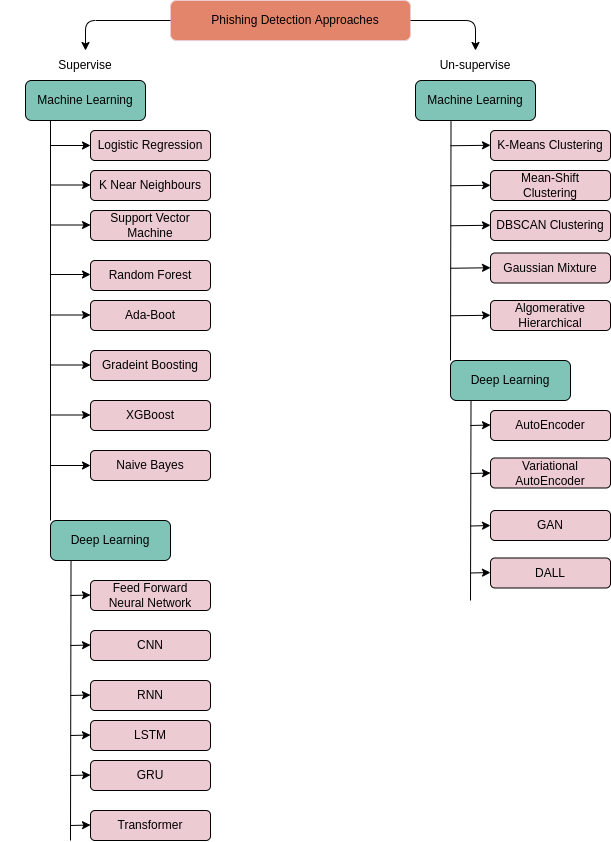
\includegraphics[width=8.5cm, height=14cm]{phishing-detection-approaches.png}
   \caption{Phishing Detection Approaches}
   \label{fig:Phishing Detection Approaches}
\end{figure}

\subsection{Logistic regression}

% (image+equation)
Logistic Regression is a classification algorithm used to assign observations to a discrete set of classes. Unlike linear
regression which outputs continuous number values, Logistic Regression transforms its output using the logistic sigmoid function to return a probability value which can then be mapped to two or more discrete classes. Logistic regression works well when the relationship in the data is almost linear
despite if there are complex nonlinear relationships between variables, it has poor performance. Besides, it requires more
statistical assumptions before using other techniques~\cite{Authors06,Authors07}.

Let’s recall the equation of simple linear regression.
 
$$\hat{y} = \beta_0 + \beta_1\ x$$

where  $\beta_0$ and $\beta_1$ are the regression coefficients and $x$ is the input feature.
In logistic regression, we pass the output of the linear regression $\hat{y}$ to a function known as the sigmoid function. The sigmoid function is of the following form:

$$h(x) = g(z) = \frac 1 {1 + e^{-z}} = \frac 1 {1 + e^{-(\beta_0 + \beta_1x)}}$$ 


\subsection{K Near Neighbors}

K-Nearest Neighbors (KNN) is one of the simplest algorithms used in machine learning for regression and classification problems which is non-parametric and lazy. In KNN
there is no need for an assumption for the underlying data distribution. KNN algorithm uses feature similarity to predict
the values of new datapoints which means that the new data point will be assigned a value based on how closely it matches the points in the training set. The similarity between records can be measured in many different ways. 

A popular choice is the Euclidean distance given by

$$d\left( p,q\right)   = \sqrt {\sum _{i=1}^{n}  \left( q_{i}-p_{i}\right)^2 }$$


Once the neighbors
are discovered, the summary prediction can be made by
returning the most common outcome or taking the average.
As such, KNN can be used for classification or regression
problems. There is no model to speak of other than holding
the entire training dataset ~\cite{Authors03}.


\subsection{Support Vector Machine}

Support vector machines (SVMs) are one of the most popular classifiers. The idea behind SVM is to get the closest point between two classes by using the maximum distance between
classes. This technique is a supervised learning model used for linear and nonlinear classification. 

\hspace*{-0.2in}
\begin{figure}[h]
   \centering
   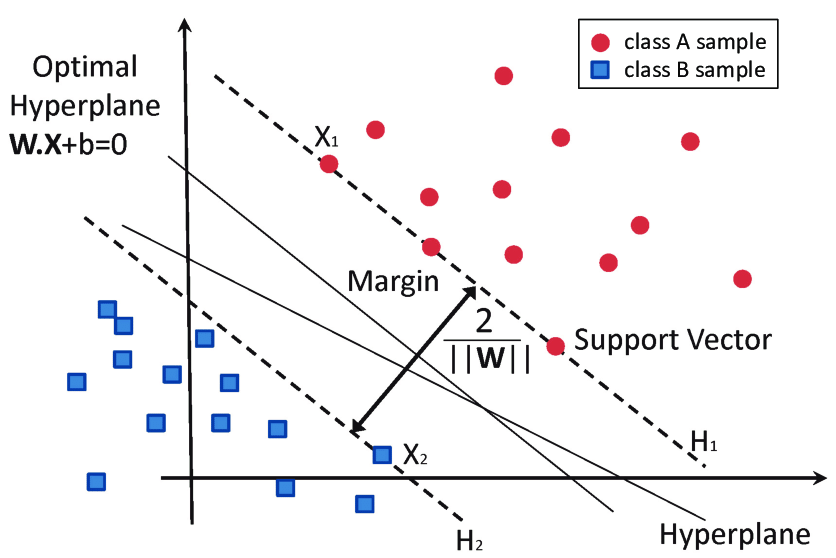
\includegraphics[width=8cm, height=5cm]{images/Support-Vector-Machine.png}
   \caption{Support Vector Machine}
   \label{fig:Support-Vector-Machine}
\end{figure}

Nonlinear classification is performed using a kernel function to map the input to a higher-dimensional feature space. Although SVMs are very powerful and are commonly used in classification, it has some
weakness. They need high calculations to train data. Also, they are sensitive to noisy data and are therefore prone to over-fitting. 


There are some of the kernels that are more widely used than others. Some of the widely used kernels are:

\subsubsection{Linear Kernel}

$$K(\mathbf{x}, \mathbf{z}) = \mathbf{x}^\intercal \mathbf{z}$$

\subsubsection{Polynomial Kernel}

    Polynomial kernel represents the similarity of vectors over the training sample in a polynomial feature space of original vectors. 

    $$K(\mathbf{x}, \mathbf{z}) = (1 + \mathbf{x}^\intercal \mathbf{z})^p$$

    Here p is the degree of the polynomial. With $p = 2$, we can have a quadratic model, with $p = 3$, cubic and so on. When $p = 1$, we have a linear kernel.

\subsubsection{Radial Basis Function Kernel (RBF kernel)}

    RBF is a very popular kernel and is used widely in many applications. RBF kernel for some feature vector $\mathbf{x}$ and $\mathbf{z}$ is defined as

    $$K(\mathbf{x}, \mathbf{z}) = e^{\left(\frac{-{\parallel \mathbf{x}-\mathbf{z} \parallel}^2}{2 \sigma^2}\right)}$$

    In the above equation, you can see the term ${\lVert\mathbf x - \mathbf z \rVert}^2$ which is the squared euclidian distance between $\mathbf{x}$ and $\mathbf{z}$.
    
    ~\cite{Authors07}.

\subsection{Random Forest}

Random forest is a popular machine learning algorithm that is widely used in data science and research. 
It is an ensemble learning method that combines multiple decision trees to create a robust and accurate model. 
In random forest, each decision tree is constructed using a subset of the available features and training data, and the final prediction is made by aggregating the results of all the trees. 
This approach helps to reduce overfitting and improve the overall performance of the model. 
Random forest can be applied to a wide range of research problems, including classification, regression, and feature selection, making it a versatile and powerful tool in data  ~\cite{Authors03,Authors07}.

\subsection{Ada-Boost}

From some aspects, Ada-boost is like Random Forest, the Ada-Boost classification like Random Forest groups weak classification models to form a strong classifier. A single
model may poorly categorize objects. But if we combine several classifiers by selecting a set of samples in each iteration and assign enough weight to the final vote, it can be good
for the overall classification. Trees are created sequentially
as weak learners and correcting incorrectly predicted samples
by assigning a larger weight to them after each round of
prediction. The model is learning from previous errors. The
final prediction is the weighted majority vote (or weighted
median in case of regression problems). In short Ada-Boost
algorithm is repeated by selecting the training set based on the
accuracy of the previous training. The weight of each classifier
trained in each iteration depends on the accuracy obtained
from previous ones .

\subsection{Gradeint Boosting}

Gradient Boosting trains many models incrementally and
sequentially. The main difference between Ada-Boost and
Gradient Boosting Algorithm is how algorithms identify the
shortcomings of weak learners like decision trees. While the
Ada-Boost model identifies the shortcomings by using high
weight data points, Gradient Boosting performs the same
methods by using gradients in the loss function. The loss func-
tion is a measure indicating how good the models coefficients
are at fitting the underlying data. A logical understanding of
loss function would depend on what we are trying to optimize.

\subsection{GBoost}

XGBoost is a refined and customized version of a Gradient
Boosting to provide better performance and speed. The most
important factor behind the success of XGBoost is its scala-
bility in all scenarios. The XGBoost runs more than ten times
faster than popular solutions on a single machine and scales
to billions of examples in distributed or memory-limited set-
tings. The scalability of XGBoost is due to several important
algorithmic optimizations. These innovations include a novel
tree learning algorithm for handling sparse data; a theoretically
justified weighted quantile sketch procedure enables handling
instance weights in approximate tree learning. Parallel and dis-
tributed computing make learning faster which enables quicker
model exploration. More importantly, XGBoost exploits out-
of-core computation and enables data scientists to process
hundreds of millions of examples on a desktop. Finally, it
is even more exciting to combine these techniques to make
an end-to-end system that scales to even larger data with the
least amount of cluster resources.

\subsection{Stacking}

This technique involves training multiple models and using the predictions of each model as input to a meta-model that makes the final prediction.

Authors in Mahmoud et al. ~\cite{othman2021empirical} proposed a stacking model using RF, KNN, DT, LDA and BNB as a base classifier(level 0), while using Logistic Regression (LR) as a meta-model (level 1) for detecting the phishing website. They used data from Grega et al. ~\cite{grega2020datasets} which contained phishing and legitimate website
instances. There are two different versions of this dataset, one with a total of 58,645(Legitimate:27,998, Phishing:30,647)instances and the second version consists of 88,647(Legitimate:58,000,Phishing:30,647) instances, with more instances with label legitimate. The datasets in total contain 111 features except for the class. The features of the datasets are divided into six groups based on: URL properties,Domain properties,URL directory properties,URL file properties,URL parameter properties,URL external metrics and resolving data. Stacking models improve the exhibition of the classifiers in terms of precision, F-measure, and ROC region.
Experimental results reveal that by utilizing sacking mod-els, they concluded that the ensemble model grants accuracy 97.49\% for dataset 1 and 98.69\% for dataset 2. 



\subsection{Artificial Neural Networks}

\hspace*{-0.9in}
\begin{figure}[h]
   \centering
   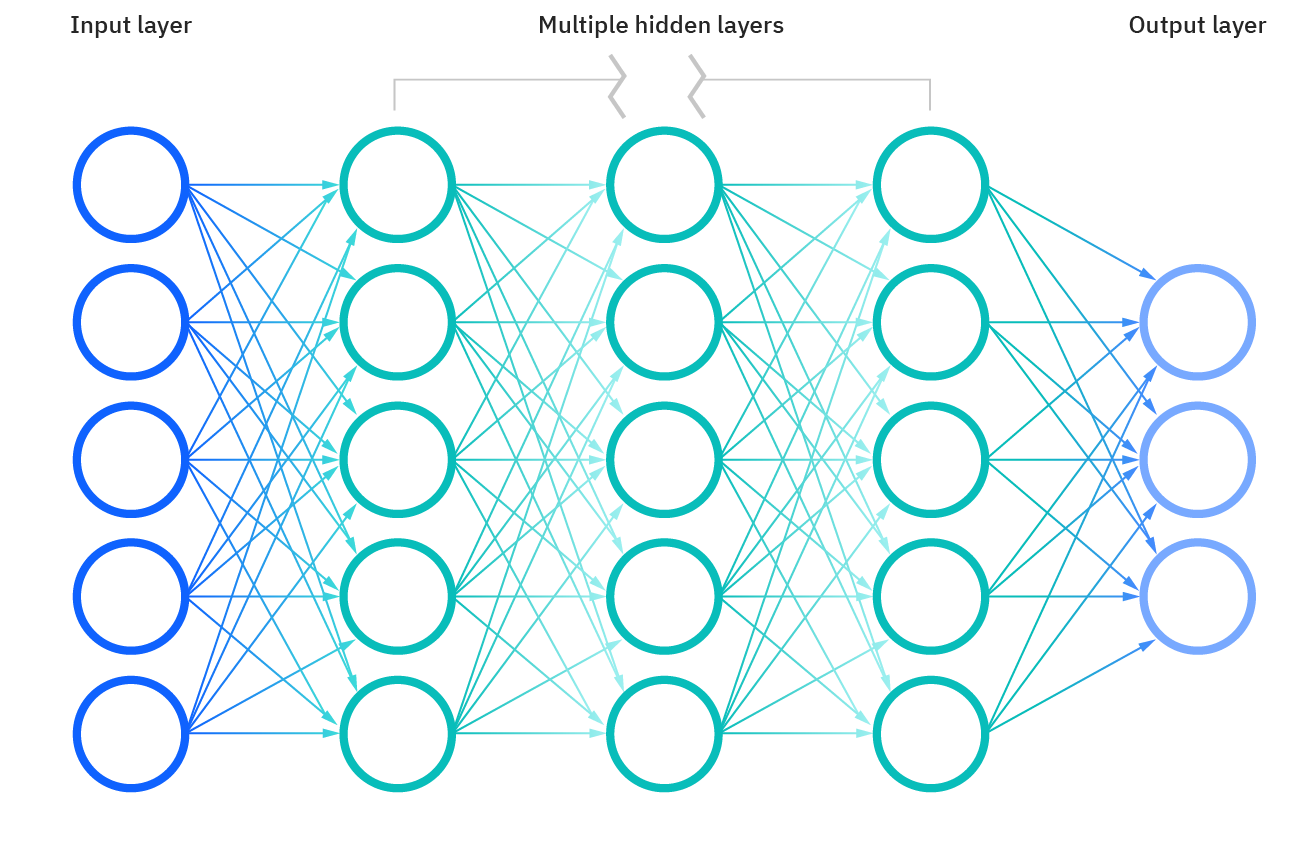
\includegraphics[width=9cm, height=6cm]{neural-network.png}
   \caption{Neural network}
   \label{fig:neural-network}
\end{figure}

Artificial neural networks (ANNS) are a learning model
roughly inspired by biological neural networks. These models
are multilayered, each layer containing several processing
units called neurons. Each neuron receives its input from
its adjacent layers and computes its output with the help
of its weight and a non-linear function called the activation
function. In feed-forward neural networks like in 3, data flows
from the first layer to the last layer. Different layers may
perform different transformations on their input. The weights
of neurons are set randomly at the start of the training and
they are gradually adjusted by the help of the gradient descent
method to get close to the optimal solution. The power of
neural networks is due to the non-linearity of hidden nodes.
As a result, introducing non-linearity in the network is very
important so that you can learn complex functions~\cite{Authors07}.

\subsection{CNN}

Convolutional Neural Networks (CNNs) are a type of deep learning algorithm that has proven to be highly effective in a wide range of computer vision tasks, such as image classification, object detection, and segmentation.

CNNs are designed to automatically learn features from input data by using convolutional layers, which apply filters to extract useful patterns and features from the input. The output of each convolutional layer is then passed through non-linear activation functions, such as ReLU, to introduce non-linearity into the network.

Pooling layers are often used after convolutional layers to reduce the spatial size of the input and increase the robustness of the network to variations in input data.

In addition to convolutional and pooling layers, CNNs also typically include fully connected layers, which map the extracted features to the final output. The entire network is trained end-to-end using backpropagation and gradient descent to minimize a given loss function ~\cite{726791,NIPS2012_4824,he2016deep,szegedy2015going,zeiler2014visualizing,srivastava2015highway,zagoruyko2016wide, simonyan2014very,zhang2017polynet,ioffe2015batch,huang2017densely,chollet2017xception}.

\subsection{RNN}

A recurrent neural network (RNN) is a type of neural network that is commonly used for processing sequential data. RNNs have a feedback loop in their architecture, which allows them to take into account previous inputs and their own previous state when making predictions.

Mathematically, an RNN can be expressed as follows:

At time step $t$, the hidden state of the RNN is denoted as $h_t$, and the output is denoted as $y_t$. The input at time $t$ is denoted as $x_t$.

The hidden state at time t is calculated as:

$h_t = f(W_hh * h_{t-1} + W_hx * x_t + b_h)$

Where $W_hh$ is the weight matrix for the hidden state, $W_hx$ is the weight matrix for the input, and $b_h$ is the bias term for the hidden state. The function $f$ is an activation function that applies a nonlinearity to the sum of the weighted inputs.

The output at time t is calculated as:

$y_t = g(W_yh * h_t + b_y)$

Where $W_yh$ is the weight matrix for the hidden state, $b_y$ is the bias term for the output, and $g$ is an activation function that applies a nonlinearity to the sum of the weighted inputs.

During training, the RNN learns the optimal values of the weight matrices and bias terms by minimizing a loss function, such as mean squared error, with respect to these parameters. This is typically done using backpropagation through time, which is an extension of the backpropagation algorithm used in standard feedforward neural networks ~\cite{rumelhart1986learning}.



\subsection{LSTM}

Long Short-Term Memory (LSTM) is a type of recurrent neural network (RNN) that has been proven to be highly effective in a wide range of sequence modeling tasks, such as natural language processing, speech recognition, and time series forecasting.

LSTM networks are designed to overcome the vanishing gradient problem of traditional RNNs, which occurs when gradients become exponentially small as they propagate back through time, making it difficult to learn long-term dependencies. LSTM networks address this issue by introducing a memory cell, which allows the network to selectively remember or forget information over time.

The memory cell is composed of three gates: an input gate, an output gate, and a forget gate. The input gate controls which information is updated and added to the memory cell, the forget gate determines which information is removed from the memory cell, and the output gate decides which information from the memory cell is used to make predictions.

The weights of the gates are learned during training using backpropagation through time, a variant of backpropagation that is used to train RNNs. The network is trained to minimize a given loss function, such as cross-entropy for classification tasks or mean squared error for regression tasks~\cite{Authors04}.

\subsection{Transformer}

The Transformer is a deep learning algorithm that was introduced in 2017 and has since become a popular choice for a wide range of natural language processing tasks, including language translation, text summarization, and question answering ~\cite{Authors05}.


\hspace*{-0.9in}
\begin{figure}[h]
   \centering
   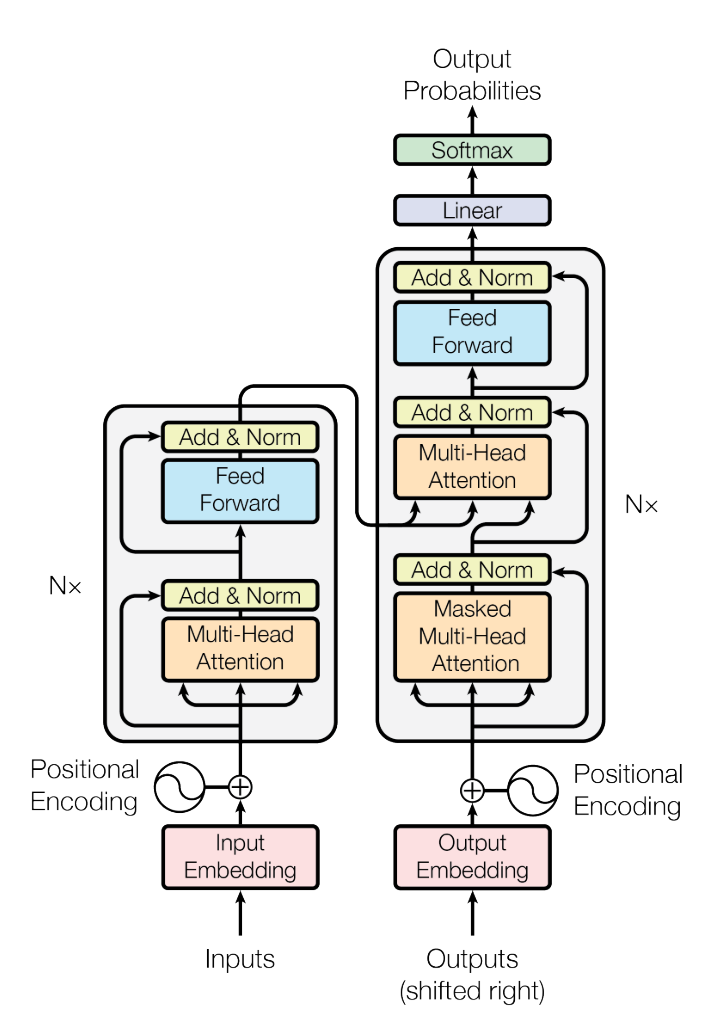
\includegraphics[width=8.5cm, height=14cm]{transformer.png}
   \caption{Transformer}
   % \label{fig:mesh1}
\end{figure}

The Transformer is based on a self-attention mechanism, which allows it to weigh the importance of different parts of the input sequence when making predictions. This is accomplished by computing an attention score for each pair of input positions, which reflects the relevance of one position to another. The attention scores are then used to compute a weighted sum of the input embeddings, which forms the output of the self-attention layer.

The Transformer also includes a multi-head attention mechanism, which allows it to attend to different aspects of the input simultaneously. This is achieved by splitting the input into multiple heads, each of which computes a separate attention score and output embedding. The outputs of the multiple heads are then concatenated and passed through a feedforward network to produce the final output.

In addition to self-attention and multi-head attention, the Transformer also includes positional encoding, which allows it to take into account the order of the input sequence. The positional encodings are added to the input embeddings to provide the network with positional information.

11. K-Means Clustering

K-means clustering is a popular machine learning algorithm used for unsupervised learning tasks, such as clustering and data segmentation. The goal of K-means is to partition a given dataset into K distinct clusters, where each cluster represents a group of similar data points.

The algorithm works by first randomly selecting K initial centroids, which serve as the centers of each cluster. Then, each data point is assigned to the cluster whose centroid is closest to it. This is done by computing the Euclidean distance between each data point and the centroids, and assigning the point to the cluster with the nearest centroid.

Once all data points have been assigned to a cluster, the centroids are recalculated as the mean of all the data points in their respective cluster. This process of assigning points to clusters and updating the centroids is repeated until convergence is reached, typically when the centroids no longer move or the change is below a specified threshold.



\section{Evaluation Matrices}
\label{sec:Evaluation Matrices}

During the testing process, performance evaluation was conducted by dividing the original dataset into training data and test data, typically 80\% and 20\% respectively. The classifier's behavior was evaluated on the testing dataset using four statistical numbers: TP (the number of correctly identified positive data points), TN (the number of correctly identified negative data points), FP (the number of negative data points labeled as positive by the classifier), and FN (the number of positive data points labeled as negative by the model). The details are presented in the table.

\begin{tabular}{c >{\bfseries}r @{\hspace{0.7em}}c @{\hspace{0.4em}}c @{\hspace{0.7em}}l}
  \multirow{10}{*}{\rotatebox{90}{\parbox{1.1cm}{\bfseries\centering actual\\ value}}} & 
    & \multicolumn{2}{c}{\bfseries Prediction outcome} & \\
  & & \bfseries p & \bfseries n & \bfseries total \\
  & p$'$ & \MyBox{True}{Positive} & \MyBox{False}{Negative} & P$'$ \\[2.4em]
  & n$'$ & \MyBox{False}{Positive} & \MyBox{True}{Negative} & N$'$ \\
  & total & P & N &
\end{tabular}


Various metrics are commonly utilized to assess performance. One of the most widely used is classification accuracy, which is calculated as the proportion of accurate predictions to the total number of predictions made:

\vspace{7pt}
accuracy = $\frac{TP+TN}
{TP+TN+FN+FP}$

\vspace{7pt}

In binary classification scenarios, it is widely recognized that random guessing would result in an accuracy of 50\%. However, in the case of imbalanced datasets, a high accuracy score does not necessarily indicate a high-quality model. For instance, consider a dataset of 10,000 websites, of which 9,000 are legitimate and 1,000 are phishing sites. Even if the prediction model did nothing, it would still achieve an accuracy score of 90\%, which could be misleading. In such cases, precision becomes an important metric. Precision is the percentage of correctly identified positive data points among those that the model predicted as positive. The number of false-positive cases (FP) indicates the rate of false warnings, which is critical in real-time phishing detection systems since it directly impacts user experience and trust.

\vspace{7pt}

Precision = $\frac{TP}
{TP + FP}$

\vspace{7pt}

Recall is another important metric, which measures the fraction of positive data points that are correctly identified as positive by the model, out of all truly positive data points. False-negative cases (FN) represent the number of phishing URLs that the model failed to detect. In the context of security systems, such as phishing detection, false-negative cases could lead to security breaches and data leakage, which could harm users significantly. Therefore, it is crucial to minimize the number of false negatives.

In such scenarios, issuing false-positive alarms, which indicate the presence of a phishing attack where none exists, can be less damaging than missing a real attack. False alarms could be annoying and may affect user experience, but it is still preferable to err on the side of caution, as missing a real attack could have severe consequences.

\vspace{7pt}

Recall = $\frac{TP}
{TP+FN}$ 

\vspace{7pt}

The F-measure or F-score is a commonly used metric that takes into account both precision and recall to provide an overall assessment of the model's performance. It is typically calculated as the harmonic mean of precision and recall and is expressed as follows:

\vspace{7pt}

$F_{\beta} = \frac{(\beta^2 + 1)\times Precision \times Recall}
{\beta^2 \times Precision + Recall} \beta \in (0, \infty) $
\vspace{7pt}

In the F-measure formula, the parameter $\beta$ is used to weigh the importance of precision and recall differently. When $\beta$ is set to 1, precision and recall are given equal importance, and the metric is referred to as F1-score. The F1-score is a widely used measure in binary classification tasks and is particularly useful when precision and recall are of equal importance. In other words, F1-score provides a balance between precision and recall, which is crucial in real-world scenarios.

The F-score does the best job of any single statistic, but all four work together to describe the performance of a classifier:

\vspace{7pt}

$F_1 = \frac{2 \times Precision \times recall}
{Precision + recall} = \frac{TP}{TP + \frac{1}{2} (FP + FN)}$

\vspace{7pt}

In addition to the evaluation metrics discussed earlier, many researchers utilize the N-fold cross-validation technique to assess the performance of phishing detection models. This technique is widely used, especially when dealing with small datasets, and involves dividing the original data samples into N subsets after shuffling the dataset randomly. One of the subsets is used for testing the model, while the remaining subsets are used for training the model. The process is repeated N times, and each time a different subset is used for testing. The results obtained from each fold are then averaged to obtain an overall performance estimate for the model. 

Typically, N is set to 10 or 5, but this can vary depending on the dataset size and complexity of the model being evaluated. The N-fold cross-validation technique is a valuable tool for evaluating model performance as it provides a more robust estimate of the model's performance, even with limited data. It also helps to reduce the risk of overfitting, which can occur when the model is trained on a small, biased subset of the data.


\begin{figure*}
   \begin{center}
      \begin{tabular}{cccc}
         \hline
         Model or Algorithm & Type & Dataset & Accuracy \\
         \hline
         Recurrent Neural Networks ~\cite{rangapur2021phish} & Single & $\begin{array}{c}46,839 \text { instances from } \\ \text { PhishTank, OpenPhish, and Common
Crawl }\end{array}$  & 99.08\\
         \hline
         BLSTM ~\cite{wang2021deep} & Single & $\begin{array}{c}245 \text { instances from } \\ \text {UCI}\end{array}$  & 95.47\\
        \hline
        CNN ~\cite{aljofey2021effective} & Single & $\begin{array}{c}83,857 \text { instances from PhishTank} \\ \text {UCI}\end{array}$  & 98.58\\
        \hline
        BERT ~\cite{elsadig2021intelligent} & Single & $\begin{array}{c}549,346 \text { instances from Kaggle} \\ \text {UCI}\end{array}$  & 96.66\\
        \hline
        VAE ~\cite{prabakaran2021enhanced} & Single & $\begin{array}{c}100,000 \text { instances from Kaggle ISCX‐URL‐2016} \\ \text {UCI}\end{array}$  & 97.45\\
        \hline

         \end{tabular}
   \end{center}
      \caption{Comparison of major state-of-the-art solutions.}
   \label{tab:ml-state-of-the-art}
   \end{figure*}

\section{Conclusion}
\label{sec:Conclusion}
Phishing is a persistent and successful security threat that impacts both individuals and targeted organizations. Despite its longevity, it remains one of the most prevalent attack methods utilized today. As attackers continue to develop increasingly sophisticated social engineering and evasion tactics, detecting and preventing these attacks becomes ever more challenging. As such, research is essential in identifying effective countermeasures.

Our research survey has revealed that there has been a significant focus on detecting phishing websites through various research efforts. Machine learning-based methods have gained popularity due to their ability to detect zero-hour attacks and handle newly discovered phishing web pages efficiently. However, to combat phishing more effectively, it is crucial to anticipate the tactics used by attackers and address the gaps in current research. In the following sections, we outline the main research gaps identified from our survey.

One of the research gaps identified is the increased use of URL shortening services by attackers to mask the true phishing URLs, which poses a challenge for list-based approaches and the management of blacklists. This also affects machine learning-based approaches as most URL features recommended in the literature become irrelevant in this scenario, resulting in the failure of detection mechanisms. Additionally, there are other unresolved issues associated with features that are related to attackers' evasion techniques. It is not enough to simply retrain a machine learning model whenever new data becomes available; there is a need to quickly identify the tactics employed by these ever-evolving attacks and automatically extract suitable features. Therefore, further research efforts should be directed towards addressing these challenges.

Exploring model explainability is another valuable area of research within the context of machine learning. Being able to understand how machine learning algorithms make decisions, such as which characteristics indicate whether a web page is legitimate or phishing, has significant implications for the design of security systems. Furthermore, investigating adversarial attacks can help improve the robustness of machine learning models.

It is also crucial to note that in order to advance the state of the art, experiments must be reproducible. This means that all implementation details must be clearly stated, and the datasets used should be made available to the public.

Lastly, we believe that education is crucial for individuals who are often the weakest link in the chain. Therefore, some form of phishing countermeasure education should be included in any solution.


{\small
\bibliographystyle{ieee_fullname}
\bibliography{egbib}
\nocite{*}
}

\end{document}
